%\documentclass{cumcmthesis}

\documentclass[withoutpreface,bwprint]{cumcmthesis} %去掉封面与编号页
\usepackage{multirow}
\usepackage{longtable}
    \title{“拍照赚钱”APP的定价模型}
    \tihao{A}            % 题号
    \baominghao{042}    % 报名号
    \schoolname{武汉大学}
    \membera{周澳}
    \memberb{傅宇千}
    \memberc{刘志豪}
    \supervisor{指导老师}
    \yearinput{2020}     % 年
    \monthinput{08}      % 月
    \dayinput{21}        % 日

\begin{document}

\maketitle
\begin{abstract}
    “拍照赚钱”APP是。

    \keywords{劳务众包\quad  聚类分析\quad   灰色关联分析\quad   多目标优化\quad  }
\end{abstract}
%\tableofcontents
\section{问题重述}
“拍照赚钱”APP是一种基于移动互联网的自助式劳务众包平台,为企业提供各种商业检查和信息搜集服务。用户注册成为APP的会员,然后从APP上领取需要拍照的任务,赚取任务标定的酬金。APP中的任务定价是其运行的核心要素,如果定价不合理,有的任务就会无人问津,而导致商品检查的失败。

附件一是一个已结束项目的任务数据,包含了每个任务的位置、定价和完成情况(“1”表示完成,“0”表示未完成);附件二是会员信息数据,包含了会员的位置、信誉值、参考其信誉给出的任务开始预订时间和预订限额,原则上会员信誉越高,越优先开始挑选任务,其配额也就越大(任务分配时实际上是根据预订限额所占比例进行配发);附件三是一个新的检查项目任务数据,只有任务的位置信息。根据以上内容提出如下四个问题:

\begin{enumerate}
    \item 研究附件一中项目的任务定价规律,分析任务未完成的原因。
    \item 为附件一中的项目设计新的任务定价方案,并和原方案进行比较。
    \item 实际情况下,多个任务可能因为位置比较集中,导致用户会争相选择,一种考虑是将这些任务联合在一起打包发布。在这种考虑下,如何修改前面的定价模型,对最终的任务完成情况又有什么影响?
    \item 对附件三中的新项目给出你的任务定价方案,并评价该方案的实施效果。
\end{enumerate}

\section{符号说明}
\begin{center}
    \begin{tabular}{cc}
        \hline
        \makebox[0.3\textwidth][c]{符号} & \makebox[0.4\textwidth][c]{意义}      \\ \hline
        $cp_k$                           & 第$k$名会员的任务完成能力             \\ \hline
        $\overline{cp_i}$                & 第$i$项任务所在网格内会员平均完成能力 \\ \hline
        $p_i$                            & 第$i$个任务的定价                     \\ \hline
        $C_i$                            & 第$i$个任务是否被完成的0-1变量        \\ \hline
        $w_{ij}$                         & 任务$i$对会员$j$的吸引度              \\ \hline
        $l_{ij}$                         & 任务$i$与会员$j$之间的距离            \\ \hline
        $choice(j)$                      & 会员$j$在预定任务时的选择             \\ \hline
        $belong(k)$                      & 完成第$k$个任务的会员                 \\ \hline
        $G_j$                            & 会员$j$的信誉值                       \\ \hline
        注:未列出及重复的符号以出现出为准
    \end{tabular}
\end{center}

\section{模型假设}
\begin{enumerate}
    \item 每个任务的工作量基本相同
    \item 会员成功预定的任务都会完成
\end{enumerate}

\section{问题一的建模与求解}

\subsection{问题一的分析}
问题一要求研究已经完成项目中的任务定价规律,并分析其中有大量问完成任务的原因。附件一给出的项目属于结果已经确定的问题,我们需要根据每个任务的定价信息与相关影响因子进行统计分析,从而建立该项目中任务的定价规律。根据经济学原理,市场上一种服务的价格与服务含有的劳动和供求关系有关;本题的数据中能构成对价格的影响因子有任务的位置、任务分布的密度、会员的位置、会员的信誉配额。其中任务与会员的距离和完成任务付出的劳动有关,会员配额、会员和任务的分布密度与供求关系有关。对于“拍照赚钱”的劳务服务,如果假设每个任务的拍照所需的劳动量大致相同,那么会员做不同的任务付出多少的区别便主要来自会员到达任务地点路程远近。对于供求关系,这应当是一个区域性的因素,也就是一个任务的定价受到的供求关系影响主要来自其周边区域,因此我们可以用任务所在区域的任务数密度、会员数密度和会员的信誉值和工作能力来反映。根据以上分析,我们提出以下四种影响任务定价的因素:任务位置、任务所在区域的任务密度,任务所在区域的会员密度,任务所在区域会员的完成能力。通过相关性分析,我们可以得到这些因素与任务定价之间的规律。再通过计算完成的任务与未完成的任务的相关度矩阵的差别,可以分析出一些任务未被完成的原因。

\subsection{建模前的数据分析}
我们首先使用Global Mapper软件把已完成的项目中的每个任务用散点图标注在地图上,用户的位置也同样标注,如下图(红色为未完成任务,绿色为已完成的任务,黄色为用户)

\begin{figure}[H]
    \centering
    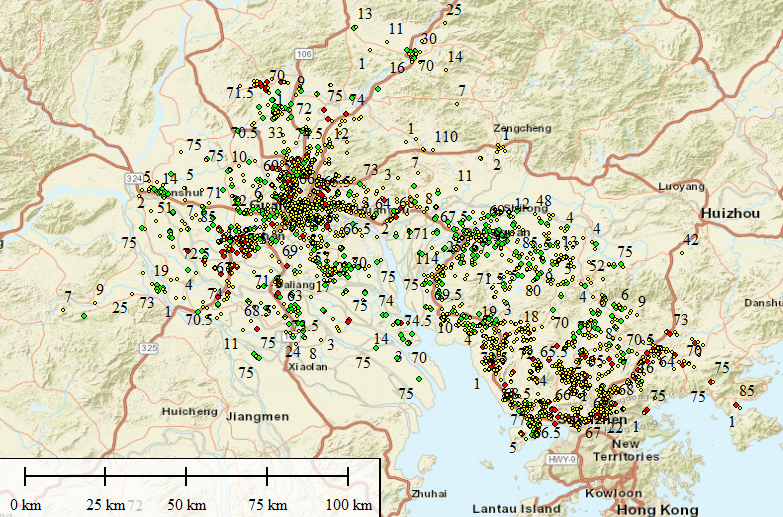
\includegraphics[width=15cm]{1.png}
    \caption{K-均值分析得到的任务中心点}
    \label{图}
\end{figure}
可以发现,任务和用户在城市和道路旁较为集中,其他地方较为分散,主要集中在广州、佛山、东莞、深圳等城市。也有几个用户的地理位置远远超出有任务的区域,应当进行去除。

我们把任务对应的定价在散点图上进行了标注,我们通过观察发现,越靠近城市繁华地带,任务和用户越密集,任务的定价也越低。我们猜想这是由于城市内交通便利,用户劳动成本低,同时用户数量多,供给过剩,因此定价低,这是与上节的分析相一致的。为了刻画任务位置对定价的影响,我们认为可以通过选定若干任务的分布中心,通过任务点位置与中心的距离远近给出定价决策的一部分。求解中心可以使用K-均值聚类分析进行。

\subsection{定价模型的建立}

\subsubsection{数据的网格化处理}
找出已完成项目中任务分布的经纬度边界,记经度区间为$[L_{min},L_{max}]$,记纬度区间为$[B_{min},B_{max}]$,将经纬度各划为50等分,则区域被划分为2500各小区域,每个小区域的经度、纬度跨度为$$\Delta L=\frac{L_{max}-L_{min}}{50},\quad \Delta B=\frac{B_{max}-B_{min}}{50}$$则对于给定的经纬坐标$(L,B)$,其所在的经纬网格的行列数为$$i=\lceil \frac{L-L_{min}}{\Delta L}\rceil,\quad j=\lceil \frac{B-B_{min}}{\Delta B}\rceil$$据此可以得出每个任务所在的网格,以及在此区域内的会员所在的网格。

\subsubsection{影响因子的确定}
根据问题分析,任务的定价有四项影响因子,即任务位置、所在网格的任务数密度、所在网格的会员数密度、所在网格的会员完成任务的能力。我们对其具体定义如下:
\begin{enumerate}
    \item 任务所在位置距离其聚类中心的距离$R_i$

          由问题分析中的描述,越接近道路和城市中心,任务定价也就越低,我们通过使用K-均值聚类分析把所有的任务分为若干组,每组有一个中心点,用任务距离中心点的距离$R_i$作为影响定价决策的一个因子,且它们之间是正相关的关系。
    \item 任务所在网格的任务数量$q_i$

          对于第$i$项任务,其所在网格内的任务总数记为$q_i$。$q_i$越大,则区域内的服务需求越多,定价与$q_i$应当成正相关关系。
    \item 任务所在网格的会员数量$Q_i$

          与上一影响因子相似,网格内会员数量越多,则服务供给越多,定价与$Q_i$应当成负相关关系。
    \item 任务所在网格的会员平均完成能力$\overline{cp_i}$

          考虑到每个会员的信誉值、预定限额和开始预定时间各不相同,只考虑会员个数并不能非常准确地反映出区域内地服务供给情况。因此我们提出会员的“任务完成能力”$cp_i$一项指标,信誉值越高、预定限额越大、开始预定时间越早的会员,其完成能力就越大。我们可以通过熵权法,用这些指标得到会员的完成能力。之后便可以计算在每个网格内的会员平均完成能力$\overline{cp_i}$。
\end{enumerate}

\subsubsection{用灰色关联分析求定价相关性}

根据以上的分析,我们得到了与任务定价相关的四个影响因子,我们通过灰色关联分析可以求解出这四个因子与定价的关联度,由此可以得到已完成项目的任务定价规律。

为了分析项目中有未完成任务的原因,可以分别把完成的任务和未完成的任务单独计算其关联度,得到灰色关联度矩阵,计算每一个影响因子的两者差值,可以分析出任务未完成可能的与定价有关的原因。

\subsection{定价模型的求解}
\subsubsection{数据网格化,计算$q_i,Q_i$}

我们首先找出附件一所给出的已完成项目中任务分布的经纬度边界:经度区间为$[L_{min},L_{max}]=[112.6,114.5]$,纬度区间为$[B_{min},B_{max}]=[22.46,23.9]$,将经纬度各划为50等分为$\Delta L=0.038,\quad \Delta B=0.0288$,由此根据模型中的公式可以确定区域内任一点所在的网格的行列数。

在将区域网格化后,可以计算出每个网格中的任务数量$q_i$和会员数量$Q_i$,由此我们便可以得到两个影响因子。

\subsubsection{K-均值聚类分析确定影响因子$R_i$}

根据对问题分析中的任务分布散点图的观察,我们发现任务大致分布在四个相对集中的区域,因此我们使用用spss的K-均值分析方法对任务的位置进行分析,将其分为四类,得到每一类的中心点。运行结果如下:
\begin{figure}[H]
    \centering
    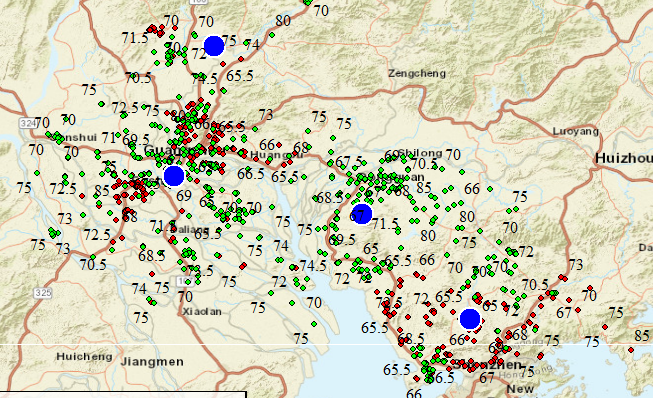
\includegraphics[width=1\textwidth]{2.png}
    \caption{K-均值分析得到的任务中心点}
    \label{图}
\end{figure}
根据分析结果,可以求出每个任务点距离它的中心点的距离$R_i$,于是我们就得到了另一个定价的影响因子。

\subsubsection{熵权法确定用户完成能力}

我们取用户的预定限额和开始预定时间这两个指标,使用熵权法确定用户的完成能力。设第$k$个会员的预定限额为$x_{k1}$,这是第一个指标。对于开始预定时间,我们观察数据可以发现最早为6:30,最晚为8:00,我们取$x_{k2}=\frac{1}{\Delta t}$作为第二个指标,其中$\Delta t$是开始预定时间与6:00相差的分钟数(若恰为6:00,则直接令$x_{k2}=1/2$。这样我们就获得了将要代入熵权法计算的两个指标$x_{k1},x_{k2}$。这两个指标与要确定的完成能力都是正相关的,我们首先把它们进行归一化:
$$x_{kj}^\prime=\frac{x_{kj}-\min_{k} \{x_{kj}\}}{\max_{k} \{x_{kj}\} - \min_{k} \{x_{kj}\}}$$
其中$x_{kj}^\prime$是第k名会员第j个指标经过归一化后的值。然后计算第j个指标下,第k名会员所占该指标的比重
$$p_{kj}=\frac{x_{kj}^\prime}{\sum_{k} x_{kj}^\prime}$$
然后计算第j项指标(j=1,2)的熵值:
$$e_j=-K\sum_{k} (p_{kj}\ln p_{kj}),\quad K=1/ln(1875)$$
计算信息熵冗余度和各项指标的权值:
$$d_j=1-e_j,\quad \lambda_j=\frac{d_j}{\sum_j d_j}$$
则一名会员的任务完成能力为
$$cp_k=\lambda_1x_{k1}+\lambda_2x_{k2}$$
经过计算,我们得到$\lambda_1=0.37021299,\quad \lambda_2=0.62978701$
再对每一个网格内的会员,计算其平均完成能力$\overline{cp_i}$,这时我们就得到了全部的定价影响因子。

\subsubsection{灰色关联分析确定关联度}

通过对任务定价与四个影响因子进行灰色关联分析,得到如下的灰色关联度矩阵:
\begin{table}[H]
    \centering
    \caption{任务定价的灰色关联度矩阵}
    \label{tab:表}
    \begin{tabular}{|c|c|c|c|c|}
        \hline
                         & $R$      & $q$      & $Q$      & $\overline{cp}$ \\ \hline
        完成的任务集合   & 0.974877 & 0.961805 & 0.948759 & 0.916587        \\ \hline
        未完成的任务集合 & 0.987225 & 0.979727 & 0.971405 & 0.958755        \\ \hline
        差值             & 0.017922 & 0.022646 & 0.042169 & 0.012348        \\ \hline
    \end{tabular}
\end{table}
通过分析,我们发现四个影响因子都对定价有很显著的影响,其中影响最大的是任务与所在区域中心点的距离,且与之成正相关。

\subsubsection{任务未完成原因的分析}
通过计算完成和未完成的任务集合对应的灰色相关度得差值,我们发现相关度相差最大的影响因子是任务所在网格的会员个数。这反映出任务不被完成的原因主要是任务定价对会员数密度不够敏感,在少有会员分布的区域,任务价格不足以吸引足够的用户去完成,因而造成了许多任务的难以完成。
\section{问题二的建模与求解}
\subsection{问题二的分析}
问题一解得的结果仅是已经结束的项目的任务定价模型,问题二进一步要求改进这一项目的定价,这实际上是一个调整定价使APP取得最大效益的优化问题。在APP开发者的角度,高效益应当是付出尽可能少的酬金,完成尽可能多的任务。为了预测项目在某种定价方式下的完成度,我们需要建立会员根据已有的定价选择任务的模型,根据题目的规定和现实生活中的经验,我们提出会员在选择任务时应当遵循以“吸引度”、信誉优先、时间次序的原则,由此可以得到在已知定价的情况下求解任务完成情况的方法。我们可以通过已完成的任务调整模型中的参数,然后可以用这一模型求解定价的优化问题。
\subsection{双目标优化模型的建立}
\subsubsection{目标函数确定}
通过对于问题的分析,新的任务定价方案与旧的定价方案相比,应该满足两个优化条件:成本更少、任务完成率更高。所以,本文将新的定价方案设计问题转化为双目标优化问题,目标函数如下:$$\left\{\begin{array}{l}
        \min \sum_{i=1}^{835} p_{i} \\
        \max \sum_{i=1}^{1835} C_{i}
    \end{array}\right.$$
其中,$p_i$为第$i$个任务的定价;$C_i$为1时,表示任务$i$被完成,$C_i$为0时,表示任务$i$未被完成。
\subsubsection{吸引度矩阵的建立}
Step1:吸引度的定义公式

在问题一未完成原因的分析求解中,本文得到了距离这个影响因子的影响作用最为显著。这表明会员在选择是否预定并完成某一单时,会重点考虑这一任务与自己的距离。同时,任务的定价直接影响到会员的收益,也会作为重要的考虑因素。

为了综合考虑这两个因素对于任务完成情况的影响,我们引入吸引度矩阵$W_{ij}$,其中矩阵中每个元素$w_{ij}$表示第$i$个任务对第$i$个任务对第$j$个会员的吸引度$(i=1,2\ldots 875,j=1,2\ldots 1875)$当任务距离会员越远,任务定价越低时,任务对会员的吸引度越低。具体定义如下:
$$w_{i j}=\sqrt{\frac{a}{l_{i j}^{2}}+b p_{i}^{2}}, \quad(\mathrm{i}=1,2 \cdots 875, \quad j=1,2 \cdots 1875)$$
其中,$l_{ij}$表示任务$i$与会员$j$之间的距离;$p_i$表示任务$i$的定价

我们假设吸引度$w_{ij}$的取值范围[0,1].。当吸引度的值接近0时,说明这个任
务对用户毫无吸引力;当吸引度的值接近于1时,说明这个任务非常具有吸引力。

Step2:参数a,b的求解

在问题一中我们曾对任务的位置分布做聚类分析,依据任务的位置信息将其
分为四类,每一类都有一个中心点。中心点的任务占据着绝对的地理优势,它对
与之距离最近的会员应当具有绝对大的吸引度,我们假设这个吸引度值为0.99。
在四个位于中心点的任务里选取两个任务,并找到与之最近的一个会员,计算两
者之间的距离,得到如下两组数据:
% Please add the following required packages to your document preamble:
% \usepackage{longtable}
% Note: It may be necessary to compile the document several times to get a multi-page table to line up properly
\begin{longtable}[c]{c|cc}
    \caption{选取的任务}
    \label{tab:my-table}       \\
    \hline
    任务号码 & A0716  & A0396  \\
    \endfirsthead
    %
    \endhead
    %
    \hline
    \endfoot
    %
    \endlastfoot
    %
    会员编号 & B0509  & B0972  \\
    $I_{ij}$ & 0.4514 & 0.2061 \\
    $P_i$    & 75     & 65.5   \\ \hline
\end{longtable}

将这两组数据代入表达式中,可以求得$a=0.01175,b=0.000164$

\subsubsection{任务吸引度的阈值确定}
在得到任务吸引度矩阵后,我们需要将每个任务对每个会员的吸引度$w_{ij}$ 与这
个任务的吸引度阈值$w_i$作比较,用以判断这个任务是否具备足够的吸引度被完
成。当吸引度大于等于阈值时,该任务具备足够的吸引度被会员领取并完成,即:
$$C_{i}=\left\{\begin{array}{ll}
        1, & w_{i j}>w_{i}      \\
        0, & w_{i j} \leq w_{i}
    \end{array}\right.$$

利用吸引度$w_{ij}$的计算公式与附件一中的任务数据计算出吸引度矩阵,当第$i$个任务被完成时,其阈值至少低于其对一个会员的吸引度;当第$i$个任务未被完成时,其阈值不低于任何其对一个会员的吸引度。阈值是作为一个判别指标与吸引度的值作比较,它的绝对值的大小并无实际意义,重要的是其相对大小,因此,阈值的确定具有一定的主观性。在这里,我们依据附件一中的任务数据,做出如下假设:
$$w_{i}=\left\{\begin{array}{l}
        \min \left\{w_{i j}\right\}, C_{i}=1 \\
        \max \left\{w_{i j}\right\}, C_{i}=0
    \end{array}\right.$$

\subsubsection{约束条件的确定}
在确定约束条件之前,我们结合题目中的条件给出如下准则:
\begin{enumerate}
    \item 最大吸引力准则:$\max \{w_{ij}\}$
    \item 竞争准则:$\max\{w_{ij}\}$
    \item 分配准则:$\text {belong}(i)=j \mid \begin{array}{l}
                  \max \left\{w_{i j}\right\} \\
                  \max \left\{G\left(n_{m}\right)\right\}
              \end{array}$,表示任务$i$分配给会员$j$
    \item 时间列准则:以第一个时间点6:30为例
          $$\begin{array}{l}
                  \qquad \operatorname{choice1}(j)=i \mid \begin{array}{l}
                      \max \left\{w_{i j}\right\}      \\
                      i=1,2 \cdots 835                 \\
                      j=1,2 \cdots, 7,14, \cdots, 1253 \\
                      \text { belong }(i)
                  \end{array} \\
              \end{array}$$
          约束条件为:
          $$\begin{array}{c}
                  50 \leq p_{i} \leq 100                                        \\
                  C_{i}=\left\{\begin{array}{l}
                      1, \quad \mathrm{W}_{i j}>w_{i} \\
                      0, \quad \mathrm{w}_{i j} \leq w_{i}
                  \end{array}\right.                 \\
                  w_{i j}=\sqrt{\frac{0.01175}{l_{i j}^{2}}+0.000164 p_{i}^{2}} \\
                  w_{i}=\left\{\begin{array}{c}
                      \min \left\{w_{i j}\right\}, C_{i}=1 \\
                      \max \left\{w_{i j}\right\}, C_{i}=0
                  \end{array}\right.                 \\
                  \operatorname{choice}(j)=k \mid \begin{array}{c}
                      w_{kj}=\min \left\{w_{i j}\right\} \\
                      i=1,2 \cdots 835, \quad j=1,2 \cdots 1875
                  \end{array}     \\
                  \begin{array}{c}
                      \qquad \operatorname{belong}(k)=n_{j} \mid \begin{array}{l}
                          w_{k n_{m}}=\max \left\{w_{i n_{m}}\right\},(m=1,2 \cdots n) \\
                          G\left(n_{j}\right)=\max \left\{G\left(n_{m}\right)\right\}(1 \leq j \leq n)
                      \end{array}
                  \end{array}
              \end{array}
          $$
\end{enumerate}

关于约束条件的说明如下:

1是关于任务定价的限定范围,这个价格范围是参照附件一中的任务定价区间大致给出的。

2表明当任务$i $对会员$j $的吸引度大于任务$i $的阈值时,任务$i$ 会被完成;当
任务$i$ 对会员j 的吸引度不大于任务$i$  的阈值时,任务$i$不会被完成。

3是上文计算出的吸引度矩阵中元素的计算公式。

4是每个任务的吸引度阈值的确定。

5是为了说明当会员$j $选择预定任务$k $时, $k $对该会员的吸引度在所有的待
选任务中是最大的,即会员会选择预约对自己吸引度最大的任务。

6是为了表明不同的会员在选择同一个任务时,信誉值最大的会员具有最大
优先度。如果有$n $个会员同时预定任务$k$ ,任务$k $最后被这$n $个会员中信誉值最
大的人成功预约。$G( j)$表示会员 $j$的信誉值。

所以,总的优化模型为:


$$\begin{aligned}
         & \begin{array}{l}
            \min \sum_{i=1}^{835} p_{i} \\
            \max \sum_{i=1}^{1835} C_{i}
        \end{array} \\
         & s.t.\quad
        \begin{cases}
             & 50 \leq p_{i} \leq 100                                        \\
             & C_{i}=\left\{\begin{array}{ll}
                1, & w_{i j}>w_{i}      \\
                0, & w_{i j} \leq w_{i}
            \end{array}\right.                \\
             & w_{i j}=\sqrt{\frac{0.01175}{l_{i j}^{2}}+0.000164 p_{i}^{2}} \\
             & w_{i}=\left\{\begin{array}{l}
                \min \left\{w_{i j}\right\}, C_{i}=1 \\
                \max \left\{w_{i j}\right\}, C_{i}=0
            \end{array}\right.                \\
             & \text {belong}(\mathrm{i})=j \mid \begin{array}{l}
                \max \left\{w_{i j}\right\} \\
                \max \left\{G\left(n_{m}\right)\right\}
            \end{array}  \\
             & \begin{array}{ll}
                \text {choice1}(j)=i \mid & \begin{array}{l}
                    \max \left\{w_{i j}\right\}      \\
                    \mathrm{i}=1,2 \cdots 835        \\
                    j=1,2 \cdots, 7,14, \cdots, 1253 \\
                    \text { belong }(\mathrm{i})
                \end{array}
            \end{array}                                    \\
            .                                                                \\
            .                                                                \\
            .                                                                \\
             & \begin{array}{l}
                \operatorname{choice} 31(j)=k\mid \begin{array}{l}
                    \max \left\{w_{i j}\right\} \\
                    j=153,165,169, \cdots, 1875 \\
                    \text { belong }(\mathrm{i})
                \end{array}
            \end{array}.
        \end{cases}
    \end{aligned}
$$
\subsection{双目标优化模型的求解}
\subsubsection{模型求解分析}
新的任务定价方案模型是在全面考虑约束条件下,建立的大型双目标优化模
型。模型的的解即长度为835 的一维定价矩阵,是通过竞争、分配、时间列准则
等个各个约束的限定,得到的满足目标函数的全局最优解。

但是模型的最优解的长度较长,约束条件复杂,如吸引度阈值、吸引度等各
个约束变量都是维度较大的矩阵,一方面即使在约束条件下对两个目标分别求解
是比较困难的,很大程度的原因在于模型中变量太多,尤其是模型的约束条件中
包含了时间列的动态变化准则,这种限制使得模型的变成非线性而且不易求解的
复杂数学模型;另一方面,从算法角度考虑, 为了得到最优的任务定价方案,
需要对任务的定价在一定范围内进行遍历并作为最外层循环,同时在内部也有吸
引度、阈值等大型数据矩阵以及内层循环遍历,进而使得算法的复杂度程指数上
升,这对算法运行时所需要的时间资源和内存资源存在很大要求。

因此综合考虑算法复杂度以及程序的运行实现,采用分布逐级优化的策略,
在算法中对模型中的约束进行一定简化,并做出适当假设,在存在一定误差之下,
得到全局最优解的近似解作为模型最优解,即任务定价方案。
\subsubsection{模型求解步骤}
Step1:预先设置任务定价

将任务的定价直接进行设定,并进行分组对比,通过得到的任务成本和任务
完成率两项指标,从而确定一种局部最优解,作为最终近似解。

Step2:吸引度矩阵确定

通过计算会员与每个任务之间的距离,根据模型二和问题一,由吸引度计算
公式得到每个任务对于每个会员的吸引度矩阵。

Step3:时间刻准则

满足不同时刻不同情况的约束条件,通过建立for 循环,将6:30 时刻转换
为编号1,依次递推,至8:00 编号31,通过循环遍历,满足不同时间可选择预
定人数不同的约束。

Step4:目标任务确定

从时刻编号1 开始,通过对释放能够预定任务的会员,相应的在该时刻能够
预定的任务中,通过遍历吸引度矩阵,找到最大吸引的任务,并记录位置。

Step5:冲突判断

判断位置记录矩阵中,是否存在数值相等的情况,即判断是否存在冲突。若
发生冲突,则对会员的信誉值进行比较,从而确定一个优先选择,即信誉高的会
员得到此次任务预定权。

Step5:方案及完成度结果

通过对时间和任务预定数的遍历,得到最终任务完成度矩阵,并输出任务完
成度数值,同时输出预先设定的任务定价矩阵。考虑到对复杂度和运行时间降低,
不采用对定价进行遍历的方式,而通过对任务定价矩阵的不同设置得到几组不同
结果,从而对比分析得到近似最优解。

\subsubsection{模型求解结果}
在对模型求解时,设定几组不同的价格调整比例,得到835 个任务的定价以
及任务完成度.由于结果数据庞大,此处只展示部分结果:

% Please add the following required packages to your document preamble:
% \usepackage{longtable}
% Note: It may be necessary to compile the document several times to get a multi-page table to line up properly
\begin{longtable}[c]{cccccc}
    \caption{定价及完成度}
    \label{tab:my-table}\\
    \hline
            & 每单定价 & 70.56 & 83.31 & 64.20 & 83.31 \\
    \endfirsthead
    %
    \endhead
    %
    \hline
    \endfoot
    %
    \endlastfoot
    %
    a=1.08  & 完成与否 & 1     & 0     & 1     & 1     \\
    b=0.99  & 成本   & \multicolumn{4}{c}{43,051}    \\
            & 完成率  & \multicolumn{4}{c}{0.75}      \\
            & 每单定价 & 72    & 85    & 65    & 85    \\
    a=1.02  & 完成与否 & 1     & 1     & 1     & 1     \\
    b=1     & 成本   & \multicolumn{4}{c}{56,926}    \\
            & 完成率  & \multicolumn{4}{c}{0.98}      \\
            & 每单定价 & 71.64 & 84.58 & 65.17 & 84.58 \\
    a=1.02  & 完成与否 & 1     & 0     & 1     & 1     \\
    b=0.995 & 成本   & \multicolumn{4}{c}{47,585}    \\
            & 完成率  & \multicolumn{4}{c}{0.83}      \\
            & 每单定价 & 71.86 & 84.83 & 65.37 & 84.83 \\
    a=1.02  & 完成与否 & 1     & 1     & 1     & 1     \\
    b=0.998 & 成本   & \multicolumn{4}{c}{54,356}    \\
            & 完成率  & \multicolumn{4}{c}{0.94}      \\ \hline
    \end{longtable}

\begin{figure}[H]
    \centering
    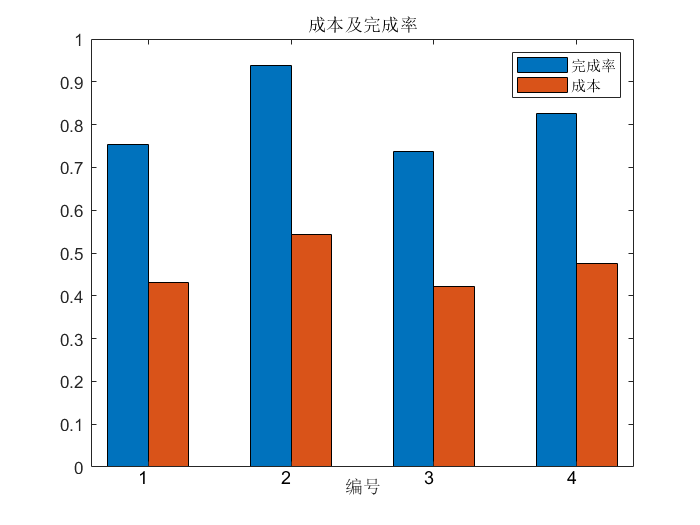
\includegraphics[width=1\textwidth]{chengben.png}
    \label{成本}
\end{figure}
在模型二给出的定价方案下,四组的成本及完成率情况如柱状图所示,其中
蓝色的值表示成本的万分之一,黄色的值表示任务完成率。综合考虑目标函数的
优化结果,选择第4组的任务定价方案作为最优定价方案。


\section{问题三的模型建立与求解}
\subsection{聚类分析确定打包方案}
问题三考虑到将位置较为集中的任务联合打包发布,从而提高了任务完成的
效率。因此,我们首先需要根据任务的位置信息判断哪些任务的位置分布较为集
中,从而确定打包方案。附件一给出的任务位置信息即为经纬度数据,首先,将
经纬度的数据作为地理位置的定量分析数据,利用聚类分析的方法,从位置分布
上对任务进行准确、细致的分类。此时,位置分布比较集中的任务会被自动归为
一类。我们将分析聚类结果的合理性,对于合理的分类,直接将此类中的任务联
合打包。对于不合理的分类,我们将对分类结果进一步调整后再打包。

Step 1:第一层聚类分析

首先,我们对聚类分析的分类数进行大致估算,由于任务总数为845 个,将
任务按照位置信息分为150 类时,平均每一类大约有5—6 个任务,这个数值比
较合理。因此,初次聚类时,将任务的位置分布分为150 类,利用Matlab 的
K-Means 命令得到的聚类分析图:

\begin{figure}[H]
    \centering
    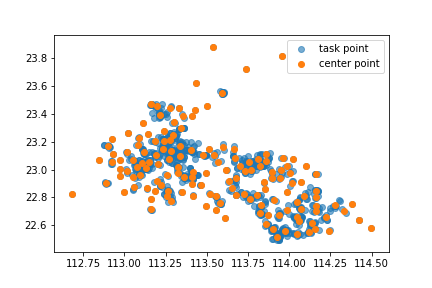
\includegraphics[width=1\textwidth]{150.png}
    \caption{K-Means聚类分析图}
    \label{}
\end{figure}

任务打包方案应当考虑两方面的问题:一是联合打包的任务应该在位置分布
上较为集中;二是一个任务包内的任务数量应当合理。我们假设一个任务包内的
任务数量取值范围为[2,15]。该聚类结果保证了一类中的任务在位置分布上较为
集中,下面来分析每个任务包中的任务数量是否符合假设。下图为每一类中任务
数量的统计图:
\begin{figure}[H]
    \centering
    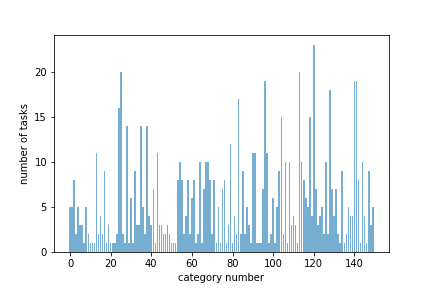
\includegraphics[width=1\textwidth]{tasks.png}
    \caption{每一类中任务数量的统计图}
    \label{}
\end{figure}

我们依据任务的位置信息将任务按照分布的集中度分成150 类,最多的类别
中有18 个任务。最少的类别中只有1 个任务。对于一类中只有1 个的任务,由
于其位置分布偏散,我们不对其做打包处理。但对于任务个数大于15 个的类别,
我们将这些任务位置信息提取出来,进行二次聚类分析。

Step 2:第二层聚类分析

我们假设当一类中任务数量不超过15 个时,这个打包方案才是合理的,在
上述聚类分析中,有九个类别中的任务数量超过了15 个.

对于这九个不合理的分类,我们在第一次分类结果的基础上,进行嵌套的聚
类分析,将它们分成两类。将这九个分类中的任务位置信息提取出来,再一次根
据其经纬度数据,利用Matlab 的K-Means 命令进行第二层聚类分析。
分别得到如下的分类图:

\begin{figure}
    \centering
    \begin{minipage}[c]{0.3\textwidth}
        \centering
        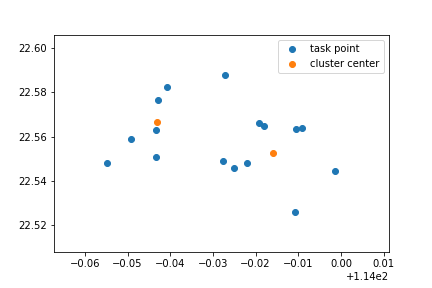
\includegraphics[width=0.95\textwidth]{24.png}
        \subcaption{第24类二次聚类图}
        \label{fig:sample-figure-a}
    \end{minipage}
    \begin{minipage}[c]{0.3\textwidth}
        \centering
        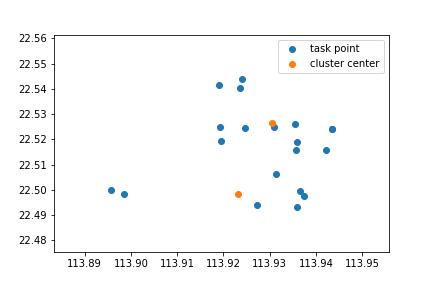
\includegraphics[width=0.95\textwidth]{25.png}
        \subcaption{第25类二次聚类图}
        \label{fig:sample-figure-b}
    \end{minipage}
    \begin{minipage}[c]{0.3\textwidth}
        \centering
        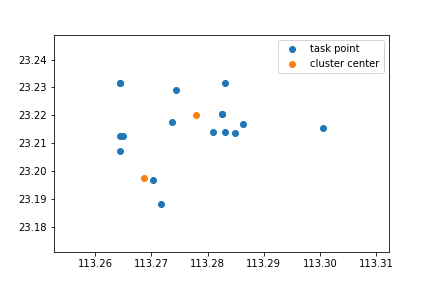
\includegraphics[width=0.95\textwidth]{83.png}
        \subcaption{第83类二次聚类图}
        \label{fig:sample-figure-c}
    \end{minipage}\\
    \begin{minipage}[c]{0.3\textwidth}
        \centering
        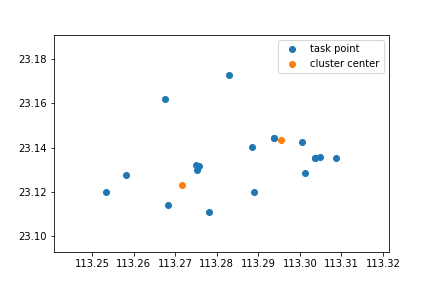
\includegraphics[width=0.95\textwidth]{96.png}
        \subcaption{第96类二次聚类图}
        \label{fig:sample-figure-a}
    \end{minipage}
    \begin{minipage}[c]{0.3\textwidth}
        \centering
        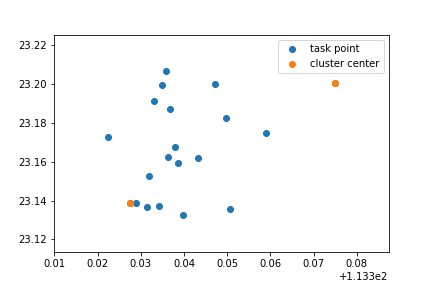
\includegraphics[width=0.95\textwidth]{113.png}
        \subcaption{第113类二次聚类图}
        \label{fig:sample-figure-b}
    \end{minipage}
    \begin{minipage}[c]{0.3\textwidth}
        \centering
        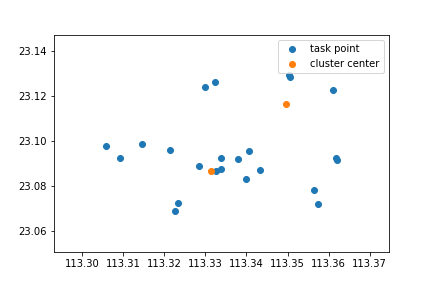
\includegraphics[width=0.95\textwidth]{120.png}
        \subcaption{第120类二次聚类图}
        \label{fig:sample-figure-c}
    \end{minipage}\\    \begin{minipage}[c]{0.3\textwidth}
        \centering
        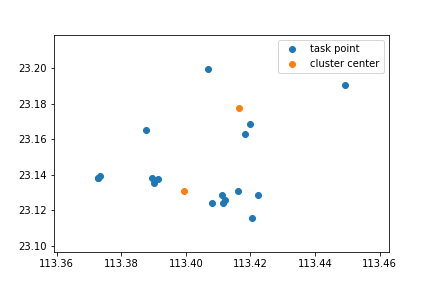
\includegraphics[width=0.95\textwidth]{128.png}
        \subcaption{第128类二次聚类图}
        \label{fig:sample-figure-a}
    \end{minipage}
    \begin{minipage}[c]{0.3\textwidth}
        \centering
        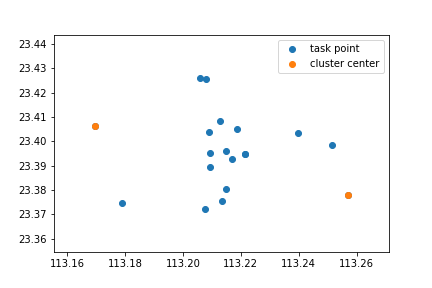
\includegraphics[width=0.95\textwidth]{140.png}
        \subcaption{第140类二次聚类图}
        \label{fig:sample-figure-b}
    \end{minipage}
    \begin{minipage}[c]{0.3\textwidth}
        \centering
        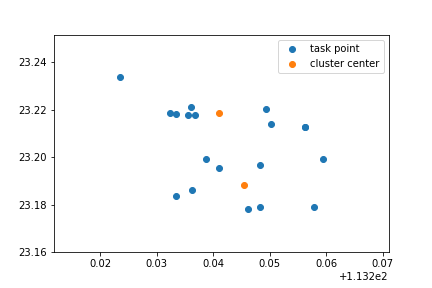
\includegraphics[width=0.95\textwidth]{141.png}
        \subcaption{第141类二次聚类图}
        \label{fig:sample-figure-c}
    \end{minipage}\\
    \caption{二重嵌套聚类分析图}
    \label{fig:sample-figure}
\end{figure}

对这九个类别进行嵌套聚类分析后,每一类别都由两个小类组成,每一小类
包含的任务数量由下面的统计表格给出:
% Please add the following required packages to your document preamble:
% \usepackage{multirow}
% \usepackage{longtable}
% Note: It may be necessary to compile the document several times to get a multi-page table to line up properly
\begin{longtable}[c]{ccc}
    \caption{嵌套聚类后任务数量}
    \label{tab:my-table}\\
    \hline
    类号                   & 新类别 & 再计数 \\ \hline
    \endfirsthead
    %
    \endhead
    %
    \multirow{2}{*}{24}  & 1   & 9   \\
                         & 2   & 7   \\ \hline
    \multirow{2}{*}{25}  & 1   & 7   \\
                         & 2   & 13  \\ \hline
    \multirow{2}{*}{83}  & 1   & 3   \\
                         & 2   & 14  \\ \hline
    \multirow{2}{*}{96}  & 1   & 8   \\
                         & 2   & 11  \\ \hline
    \multirow{2}{*}{113} & 1   & 12  \\
                         & 2   & 8   \\ \hline
    \multirow{2}{*}{120} & 1   & 7   \\
                         & 2   & 15  \\ \hline
    \multirow{2}{*}{128} & 1   & 5   \\
                         & 2   & 13  \\ \hline
    \multirow{2}{*}{140} & 1   & 12  \\
                         & 2   & 7   \\ \hline
    \multirow{2}{*}{141} & 1   & 10  \\
                         & 2   & 9   \\ \hline
    \end{longtable}
嵌套聚类分析后,每一类别的任务数量符合要求,此时得到的分类方案合理。


Step 3:确定任务打包方案

根据上述两次基于任务位置分布的聚类分析结果,我们将位置分布较为集中
的任务联合打包,同时保证每一个任务包内的任务数量不多于15 个,得到了一
个合理、准确的任务打包方案。

将一个任务包里的多个任务看做一个整体,与其它未被打包的任务同为一个
任务,经过联合打包处理过后的任务数量由835 个变为154 个。

\subsection{改进后的双目标定价优化模型}
利用聚类分析我们可以得到任务的打包方案,将位置分布较为集中的多个任
务进行联合打包,并将其看做一个整体,即为一个任务包,不论是没有打包的单
个任务还是一个任务包,我们在进行分析时都将其看做是一个任务。在问题二给
出的双目标优化定价模型中我们定义了一个吸引度矩阵,给出了矩阵中每一个元
素的计算公式,即:
$$w'_{i j}=\sqrt{\frac{0.01175}{l_{i j}^{2}}+0.000164 p_{i}^{2}}, \quad(\mathrm{i}=1,2 \cdots 835, \quad \mathrm{j}=1,2 \cdots 1875)$$
在对位置分布较为集中的多个任务进行打包处理后,任务总数会改变,需要
重新计算每个任务距离每位会员的距离,调整任务定价,从而吸引度矩阵的值会
发生相应变化。

经过聚类分析组合成的每个任务包都有一个中心点,我们将每个任务包的中
心点的经纬度坐标看作是这个任务的位置信息,计算每个任务包中心点与每位会
员之间距离。而对于那些位置分布较为松散,没有被打包处理的单个任务而言,
它们距离每位会员的距离不会发生改变。至此,我们得到打包处理后的距离矩阵
$L'_{ij}$,其中每个元素$l'_{ij}$表示任务$i $或者任务包$i $与会员$j $之间的距离。

经调整后的任务吸引度矩阵$W'_{ij}$中每个元素的表达式为:
$${w'}_{i j}^{\prime}=\sqrt{\frac{0.01175}{{l'}_{i j}^{\prime 2}}+0.000164 p_{i}^{2}}, \quad(\mathrm{i}=1,2 \cdots 154, \quad \mathrm{j}=1,2 \cdots 1875)$$

在利用双层嵌套聚类分析给出合理的打包方案后,任务总数变为154,这154
个任务预定过程依旧遵循问题二中的问题三是在对任务进行联合打包操作后,
对问题二的定价优化函数模型进行修改,在将多个位置比较集中的任务联合打包
发布的前提下,给出最优定价方案。因此,问题三实质上依旧是一个优化问题,
并且目标函数与问题二中模型的一致,通过改变约束条件来改变目标函数的求解
结果,从而修改前面的定价模型。得到在问题三的约束下的最优定价模型。

在修改后的优化模型中,发布的任务数量、距离矩阵、吸引度矩阵与
阈值均发生改变,建立起如下修改后的双目标定价优化模型:
$$\begin{aligned}
    & \begin{array}{l}
       \min \sum_{i=1}^{154} p_{i} \\
       \max \sum_{i=1}^{154} C_{i}
   \end{array} \\
    & s.t.\quad
   \begin{cases}
        & 50 \leq p_{i} \leq 100                                        \\
        & C_{i}=\left\{\begin{array}{ll}
           1, & w'_{i j}>w'_{i}      \\
           0, & w'_{i j} \leq w'_{i}
       \end{array}\right.                \\
        & {w'}_{i j}=\sqrt{\frac{0.01175}{{l'}_{i j}^{2}}+0.000164 p_{i}^{2}} \\
        & {w'}_{i}=\left\{\begin{array}{l}
           \min \left\{w'_{i j}\right\}, C_{i}=1 \\
           \max \left\{w'_{i j}\right\}, C_{i}=0
       \end{array}\right.                \\
        & \text {belong}(\mathrm{i})=j \mid \begin{array}{l}
           \max \left\{{w'}_{i j}\right\} \\
           \max \left\{G\left(n_{m}\right)\right\}
       \end{array}  \\
        & \begin{array}{ll}
           \text {choice1}(j)=i \mid & \begin{array}{l}
               \max \left\{{w'}_{i j}\right\}      \\
               \mathrm{i}=1,2 \cdots 154        \\
               j=1,2 \cdots, 7,14, \cdots, 1253 \\
               \text { belong }(\mathrm{i})
           \end{array}
       \end{array}                                    \\
       .                                                                \\
       .                                                                \\
       .                                                                \\
        & \begin{array}{l}
           \operatorname{choice} 31(j)=k\mid \begin{array}{l}
               \max \left\{{w'}_{i j}\right\} \\
               j=153,165,169, \cdots, 1875 \\
               \text { belong }(\mathrm{i})
           \end{array}
       \end{array}.
   \end{cases}
\end{aligned}
$$
\subsection{模型的求解}
\subsubsection{模型求解分析}
问题三的模型建立在问题二的模型之上,仍然考虑对模型中的约束进行一定
简化,并做出适当假设,得到全局最优解的近似解作为模型最优解。问题三模型
任务安排采用打包分配模式,首先通过聚类把类似的任务聚成一类,从而降低了
任务的维度。新的任务数即打包数量影响着任务阈值、吸引度矩阵等变量,通过
聚类打包求得新的任务情况,从而套用问题二的算法,对部分变量和维度进行修
改,经过遍历得到更优结果。
\subsubsection{模型求解步骤}
Step1:聚类打包

通过聚类算法,对任务进行分类,相似度较高的任务归为一类成为一个任务
包。部分个体未归入聚类类别的单独视为一个任务包。

Step2:预先设置任务定价

采用与问题二不同的定价模式。根据聚类,分别得到每个打包任务中单个任
务的最高、平均、最低价格,从而分为三种情况,分别将每个包中最高、平均、
最低作为打包任务的整体平均值。

Step3:吸引度矩阵更新

更新得到计算会员与每个打包之间的距离,并根据模型二,由吸引度计算公
式对每个任务对于每个会员的吸引度矩阵重新进行计算。

Step4:冲突判断

判断位置记录矩阵中,是否存在数值相等的情况,即判断是否存在冲突。若发生冲突,则对会员的信誉值进行比较,从而确定一个优先选择,即信誉高的会员得
到此次任务预定权。

Step5:方案及完成度结果

通过对时间和任务预定数的遍历,得到最终任务完成度矩阵,并输出任务完成度
数值,同时输出预先设定的任务定价矩阵。考虑到对复杂度和运行时间降低,不
采用对定价进行遍历的方式,而通过对任务定价矩阵的不同设置得到几组不同结
果,从而对比分析得到近似最优解。
\subsection{模型求解结果}
在对模型求解时,设定几组不同的价格调整比例,得到835 个任务的定价以
及任务完成度,由于结果数据庞大,此处只展示部分结果:
% Please add the following required packages to your document preamble:
% \usepackage{longtable}
% Note: It may be necessary to compile the document several times to get a multi-page table to line up properly
\begin{longtable}[c]{cccccc}
    \caption{}
    \label{tab:my-table}\\
    \hline
            & 每单定价 & 69.80 & 69.55 & 72.22 & 71.68 \\
    \endfirsthead
    %
    \endhead
    %
    \hline
    \endfoot
    %
    \endlastfoot
    %
    a=1.1   & 完成与否 & 1     & 0     & 1     & 1     \\
    b=0.99  & 成本   & \multicolumn{4}{c}{45,762}    \\
            & 完成率  & \multicolumn{4}{c}{0.76}      \\
            & 每单定价 & 70.15 & 69.90 & 72.22 & 71.68 \\
    a=1.1   & 完成与否 & 1     & 1     & 1     & 1     \\
    b=0.995 & 成本   & \multicolumn{4}{c}{52,403}    \\
            & 完成率  & \multicolumn{4}{c}{0.87}      \\
            & 每单定价 & 70.15 & 69.90 & 75.50 & 74.94 \\
    a=1.15  & 完成与否 & 1     & 1     & 1     & 1     \\
    b=0.995 & 成本   & \multicolumn{4}{c}{53,563}    \\
            & 完成率  & \multicolumn{4}{c}{0.87}      \\
            & 每单定价 & 69.80 & 69.55 & 75.50 & 74.84 \\
    a=1.15  & 完成与否 & 1     & 1     & 0     & 1     \\
    b=0.99  & 成本   & \multicolumn{4}{c}{46,921}    \\
            & 完成率  & \multicolumn{4}{c}{0.76}      \\ \hline
    \end{longtable}
\section{问题四的建模与求解}

\section{模型总结}
\subsection{模型一}

优点:

1.从定性与定量的两个角度分析任务的定价规律,通过图像直观清晰地观察定价
的定性规律,再定量给出影响因子对定价规律的影响程度。

2.利用空间数据离散化的思想,将任务分布的经纬度区间划分为等面积的网格区
域,便于统计每一个网格区间内的任务与会员的相关数据,计算影响因子的数值。

3.对任务的位置信息进行K-Means 分析,将其划分为四类,得到每一个任务到相
应中心点的距离,相当准确、细致地定量分析了任务与中心点之间的距离这个影
响因子对定价规律的影响。

4.灰色关联分析很好地避免了多元回归分析中拟合度较低的问题,系统地定量分
析了四大影响因子对任务定价规律的影响。

缺点:

1.各影响因子之间不可避免地存在相关性,未能充分考虑到影响因子之间的交互
作用。

2.考虑每个网格区域内的任务与会员数据时,对于分布在网格区域边界周围的任
务而言,会影响定价影响模型的精度。

\subsection{模型二}

优点:

5.建立任务对用户的吸引度矩阵,通过计算与比较得到每一个任务的吸引度阈值,
提供了每一个任务能否被完成的判断准则。

6.在设立模型约束条件时,不仅从企业的目标优化角度考虑,同时考虑到每位会
员不同的信誉值以及与之对应的预定开始时间和预定限额,模型的建立十分符合
任务被预定的实际情形。

7.以6:30 作为开始时间点,以3 分钟作为间隔,以时间为顺序考虑每个时间点
的情形,思考深入而全面。

缺点:

3.考虑的情况太过庞杂,需要获取的数据量十分巨大,给模型的求解与算法的实
现带来了相当大的困难。

\subsection{模型三}

优点:

8.在考虑任务的位置分布时,利用位置的经纬度坐标进行聚类分析,使任务的打
包方案设计准确又全面。

9.对于第一次聚类分析打包的任务过多的情况,将这一类里的任务提取出来做二
次聚类分析。运用二重嵌套聚类分析的方法,想法大胆又合理,保证打包方案的
全面性与可行性。

10.将设计的打包方案与问题二中的优化定价模型相结合来求解问题三,使得每
一问之间环环相扣、层层递进。

缺点:

5.在任务分布稀疏的地区,聚类分析得到的一类任务包中的任务位置并非那么集
中,对定价方案的设计存在一定影响。

4.吸引度矩阵中元素的计算公式以及吸引度阈值的确定存在一定的主观性。

\subsection{模型四}

优点:

1.问题四中新项目的定价利用问题二、三中的定价模型与打包机制,利用问题三
中的定价方案数据,通过BP 神经网络预测法给出新项目的定价方案,想法新颖
大胆,又具有合理性。

2.新项目的任务定价方案确定是基于问题一、二、三的分析与结论的,很好地检
验了前面模型的合理性与正确性。

缺点:

1.利用BP 神经网络预测出新的任务定价时,会忽略其他一些因素对定价的影响。

\begin{thebibliography}{9}%宽度9
    \bibitem[1]{1}
杜剑平,韩中庚,“互联网+”时代的出租车资源配置模型[J],数学建模及
    其应用,2015,4(04):40-49+85. [2017-09-17].
    \bibitem[2]{2}
    卓金武,李必文,魏永生,秦健.MATLAB 在数学建模中的应用,北京:北京
    航空航天大学出版社,2014.9
    \bibitem[3]{3}
    姜启源,谢金星,叶俊,数学模型(第四版),北京:高等教育出版社,2011.1
\end{thebibliography}

\begin{appendices}
\end{appendices}
\end{document}